\documentclass[compress]{beamer}
\usepackage{ifthen}

\title{Alignment Monitoring}
\author{Jim Pivarski}
\institute{Texas A\&M University}
\date{23 March, 2007}

\setbeamertemplate{navigation symbols}{}
\setbeamertemplate{headline}{\includegraphics[height=1 cm]{../cmslogo} \hspace{0.1 cm} \includegraphics[height=1 cm]{../tamulogo} \hfill
\begin{minipage}{9 cm}
\vspace{-0.75 cm} \small
\begin{center}
\ifthenelse{\equal{\insertpagenumber}{1}}{}{\insertsection}
\end{center}
\end{minipage} \hfill
\begin{minipage}{1 cm}
\vspace{-0.75 cm} \small
\begin{center}
\ifthenelse{\equal{\insertpagenumber}{1}}{}{\insertpagenumber/\pageref{numpages}}
\end{center}
\end{minipage}}

%% \xdefinecolor{verylightgray}{rgb}{0.95,0.95,0.95}
%% \beamertemplateshadingbackground{verylightgray}{white}
\xdefinecolor{dkblue}{rgb}{0.1,0.1,0.7}

\begin{document}
\frame{\titlepage}
\section*{Alignment Monitoring --- Jim Pivarski}

\begin{frame}
\frametitle{Trying to include all suggestions}
\begin{minipage}{1.1\linewidth}
\begin{enumerate}\setlength{\itemsep}{0.3 cm}
\item DQM-based monitoring upstream of alignment process
\uncover<2->{\begin{itemize}
\item Monitors pre-loaded alignment (whatever is in HLT)
\item Compares with reference/reports an error if something's wrong
\item Most urgent: needs to be in CSA07 (not yet started)
\end{itemize}}
\item Sanity checks in AlignmentProducer
\uncover<3->{\begin{itemize}
\item Coverage, convergence, iterative improvement in residuals
\item Needs to be in AlignmentProducer's loop to book new histograms with each iteration
\end{itemize}}
\item Geometry validation: have the chambers moved?
\uncover<4->{\begin{itemize}
\item Reads multiple geometries to look at differences/time dependence
\item Does not loop over tracks; reads geometries {\it only}
\end{itemize}}
\item Validation in reconstructed data: does the resolution improve?
\uncover<5->{\begin{itemize}
\item Confirms alignment in data (e.g.\ we installed the right geometry)
\item Same functionality as \textcolor{dkblue}{1}: compare to reference, same plots(?)
\end{itemize}}
\end{enumerate}
\end{minipage}
\end{frame}

\begin{frame}
\frametitle{Where these fit into the big picture}
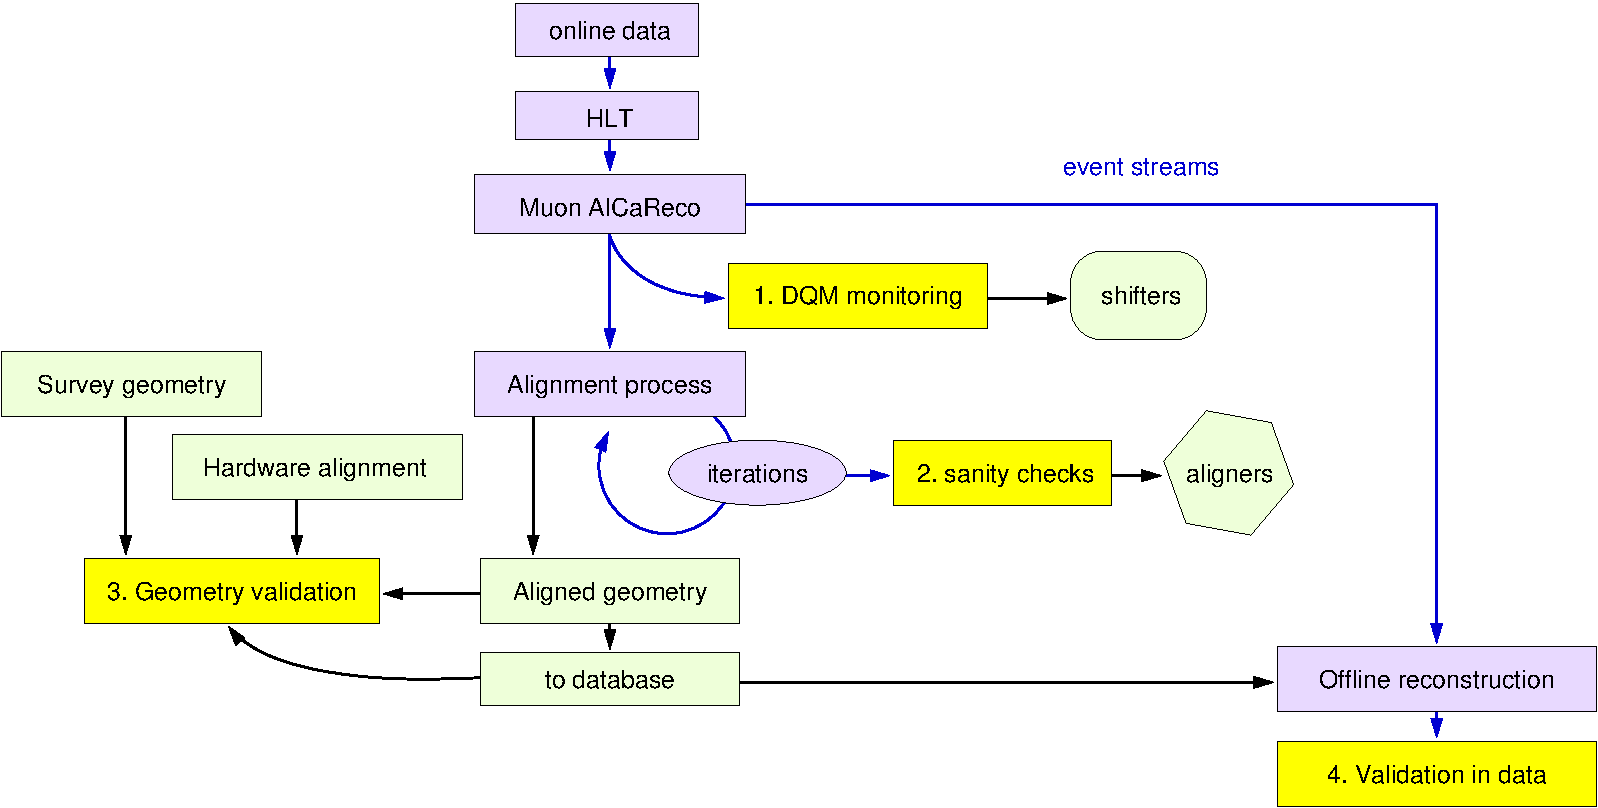
\includegraphics[width=\linewidth]{loops}
\begin{itemize}
\item Histogram-filling modules attach to existing event streams; they don't require new loops
\end{itemize}
\end{frame}

\begin{frame}
\frametitle{Plots that can be attached to any track loop (1, 2, and 4)}
\begin{minipage}{1.1\linewidth}
\begin{itemize}\setlength{\itemsep}{0.75 cm}
\item $J/\psi$, $\Upsilon$, $Z$ dimuon mass spectrum
\item $p_T$ for selected events
\item Residuals versus everything ($R$, $\phi$, $Z$, chamber-by-chamber?)
\item Overlap plots for physically overlapping chambers
\end{itemize}
\end{minipage}
\begin{columns}
\column{0.4\linewidth}
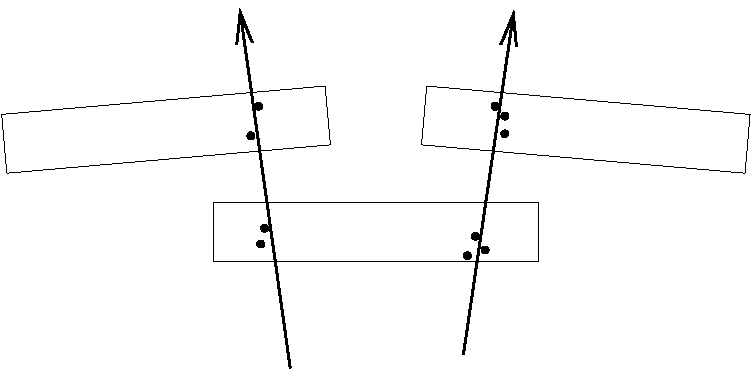
\includegraphics[width=\linewidth]{overlap_plots}
\column{0.55\linewidth}
$\mbox{residual}_{\mbox{\scriptsize chamber 1}} - \mbox{residual}_{\mbox{\scriptsize chamber 2}}$

\vspace{0.5 cm}
(track cancels, effectively a ``ruler'' curved by the $\vec{B}$ field)
\end{columns}
\end{frame}

\begin{frame}
\frametitle{Plots specifically for AlignmentProducer iterations}

\begin{tabular}{p{0.45\linewidth} p{0.45\linewidth}}
\begin{minipage}{\linewidth}
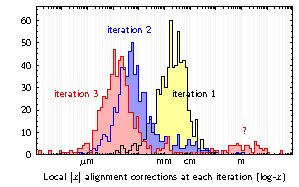
\includegraphics[width=\linewidth]{three_iterations_really}
\end{minipage} &
\begin{minipage}{\linewidth}
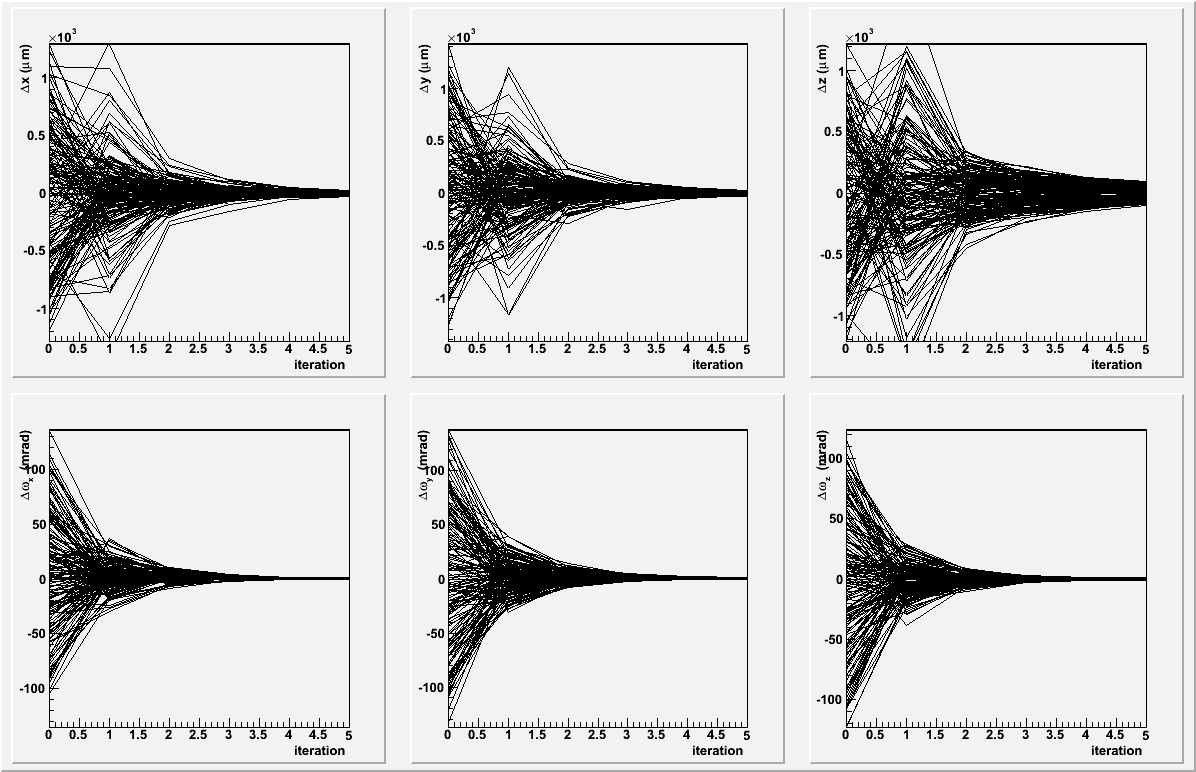
\includegraphics[width=\linewidth]{shifts_vs_iter_survey.png}
\end{minipage} \\ & \\
\begin{minipage}{\linewidth}
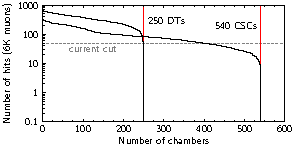
\includegraphics[width=\linewidth]{coverage}
\end{minipage} &
\begin{minipage}{1.2\linewidth}
\begin{itemize}
\item Is the procedure converging (HIP mostly)?
\item Are we missing any chambers (all algos)?
\item Histograms need to know which iteration we're on
\end{itemize}
\end{minipage}
\end{tabular}
\end{frame}

\begin{frame}
\frametitle{If there's enough memory in the budget\ldots}

  $r_x$ vs $x$, $y$ for {\it every} DT/CSC, and $r_y$ vs $y$ for
  {\it every} CSC

  \vspace{-0.75 cm}
  \begin{center}

    \begin{tabular}{p{0.33\linewidth} p{0.33\linewidth} p{0.33\linewidth}}
      \begin{minipage}{\linewidth}
      \end{minipage} &
      \begin{minipage}{\linewidth}
	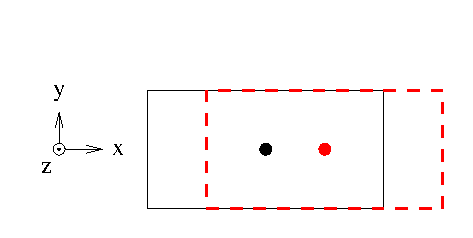
\includegraphics[width=0.8\linewidth]{dof_x}
      \end{minipage} &
      \begin{minipage}{\linewidth}
	\hspace{-0.8 cm}
	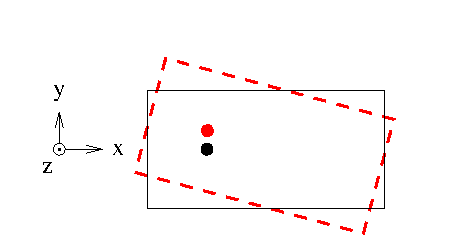
\includegraphics[width=0.8\linewidth]{dof_phiz}
      \end{minipage} \\
      \begin{minipage}{\linewidth}
      \end{minipage} &
      \begin{minipage}{\linewidth}
	\hspace{0.4 cm}
	\small $x$: offset in $r_x$
      \end{minipage} &
      \begin{minipage}{\linewidth}
	\hspace{-0.6 cm}
	\small $\phi_z$: $r_x$ linear in $y$
      \end{minipage} \\
      & & \\
      \begin{minipage}{\linewidth}
	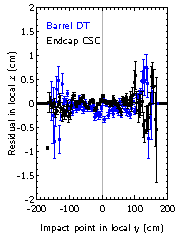
\includegraphics[width=\linewidth]{init_xresid_vs_y}
      \end{minipage} &
      \begin{minipage}{\linewidth}
	\hspace{-0.7 cm}
	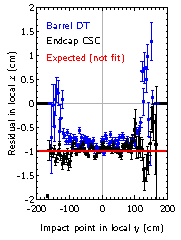
\includegraphics[width=\linewidth]{x_xresid_vs_y}
      \end{minipage} &
      \begin{minipage}{\linewidth}
	\hspace{-1.4 cm}
	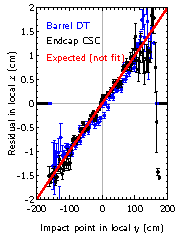
\includegraphics[width=\linewidth]{phiz_xresid_vs_y}
      \end{minipage}
    \end{tabular}
  \end{center}
\end{frame}

\begin{frame}
\frametitle{Geometry Validation (early development)}

Reads two geometries and takes their difference: $\Delta \vec{p}$

\vfill

\begin{columns}
\column{0.7\linewidth}
\only<1>{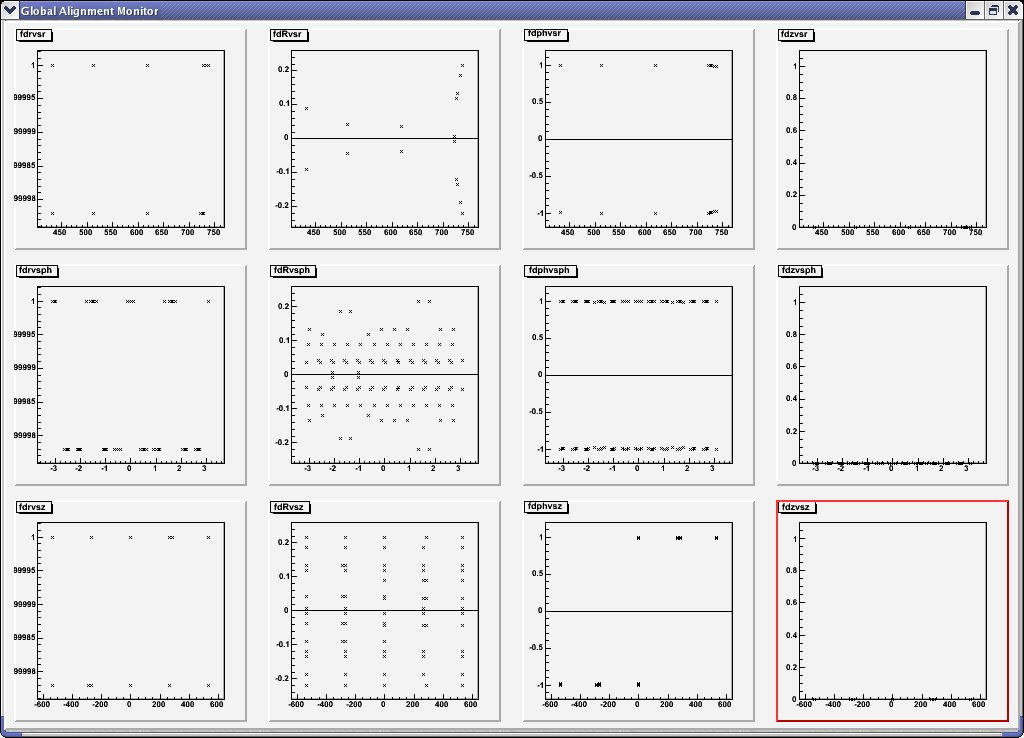
\includegraphics[width=\linewidth]{TDplots_03_22.jpg}}\only<2>{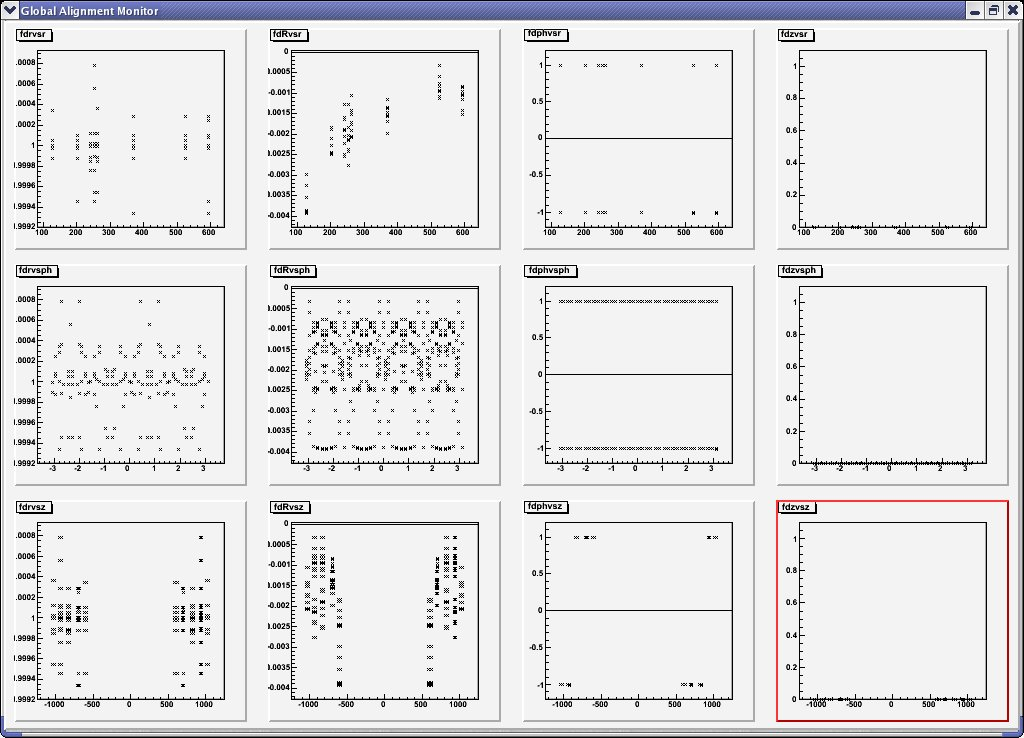
\includegraphics[width=\linewidth]{SCSplots_03_22.jpg}}
\column{0.1\linewidth}
vs.\ $R$ \\

\vspace{1.5 cm}
vs.\ $\phi$ \\

\vspace{1.5 cm}
vs.\ $Z$ \\
\end{columns}

\vfill \small \hspace{0.7 cm} $|\Delta \vec{p}|$ \hspace{0.8 cm} $\Delta \vec{p}\cdot\hat{R}$ \hspace{0.8 cm} $\Delta \vec{p}\cdot\hat{r\phi}$ \hspace{0.8 cm} $\Delta \vec{p}\cdot\hat{Z}$ \hfill (\only<1>{DT}\only<2>{CSC})
\end{frame}

\begin{frame}
\frametitle{Validation in Reconstructed Data}
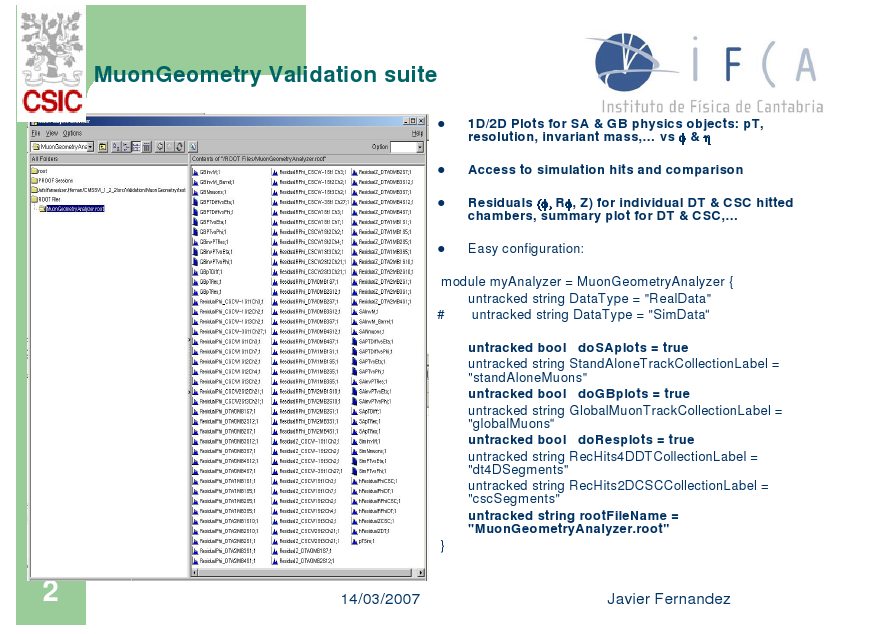
\includegraphics[width=\linewidth]{javier1.png}
\end{frame}

\begin{frame}
\frametitle{Validation in Reconstructed Data}
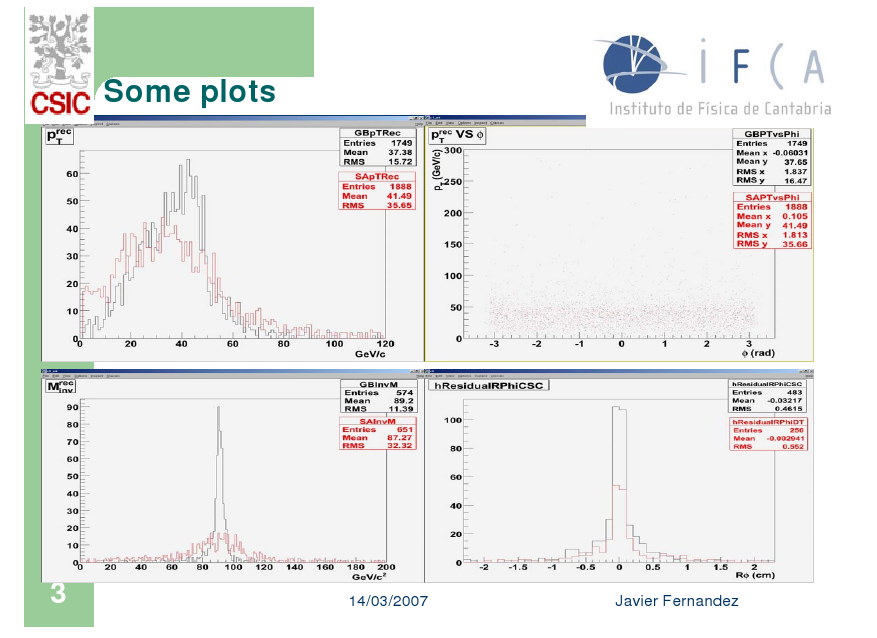
\includegraphics[width=\linewidth]{javier2.png}
\end{frame}

\begin{frame}
\frametitle{Who will do what?}
\begin{enumerate}\setlength{\itemsep}{0.75 cm}
\item DQM-based monitoring \hfill \textcolor{dkblue}{Javier Fernandez?}
\item Sanity checks in AlignmentProducer \hfill \textcolor{dkblue}{Jim Pivarski?}
\item Geometry Validation \hfill \textcolor{dkblue}{Dmitry Yakorev, Jim Pivarski}
\item Validation with reconstructed tracks \hfill \textcolor{dkblue}{Javier Fernandez}
\end{enumerate}

\vfill Discussion?

\label{numpages}
\end{frame}

\end{document}
